\section{The Key Party}

We held our key party with Lachlan, Adam and Tony to sign each others PGP certificates with our certificate authorities. We drew the short straw by having to sign 3. We used our local CA which was created with the basic constraint extension performed on the generation of this certificate, evident by the below screenshot.

\begin{figure}[hbt!]
	\centering
      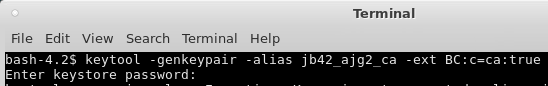
\includegraphics[width=0.7\textwidth]{imgs/x509_creation/ca_x509_creation.PNG} \\
	\caption{Generating X.509 CA certificate with Antonio's details}
	\label{fig:x509_creation:ca}
    \noindent\makebox[\linewidth]{}
\end{figure}

\noindent As all the steps for the group signing are repetitive, we will run through the signing of a certificate. There is evidence at the end of the section to display all three PGP files were signed. We imported each member's PGP private key \textbf{*.asc} file and confirmed their input as evident by the screenshot below.

\begin{figure}[hbt!]
	\centering
      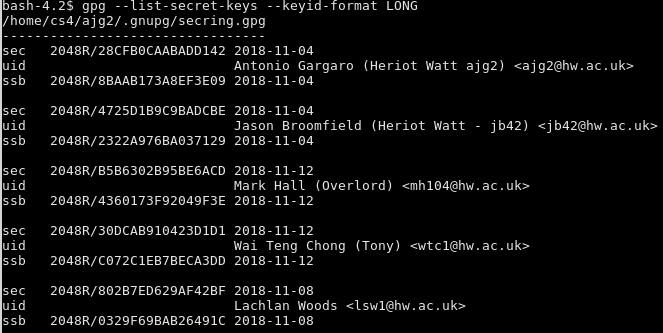
\includegraphics[width=\textwidth]{imgs/key_signing/PGP_Key_List.PNG} \\
	\caption{Listing all secret keys in our GPG key ring}
	\label{fig:key_part:keys_list}
    \noindent\makebox[\linewidth]{}
\end{figure}

\noindent We then edited the private key which allowed us to sign the key and confirm our changes.
We then confirmed the changes by quitting the GPG, and then listed each specific signature using their key specifiers. Checking each file is evident by figure \ref{fig:key_part:keys_list}.

\begin{figure}[hbt!]
	\centering
      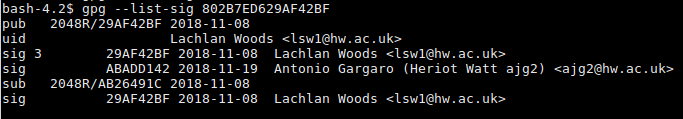
\includegraphics[width=\textwidth]{imgs/key_signing/lachlan_sign.png} \\
      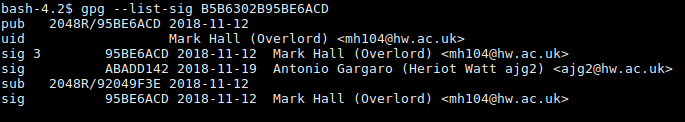
\includegraphics[width=\textwidth]{imgs/key_signing/Mark_sign.png} \\
      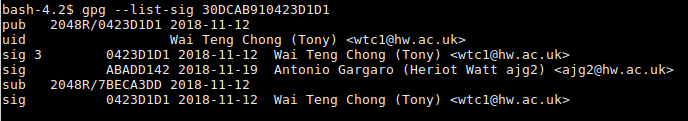
\includegraphics[width=\textwidth]{imgs/key_signing/Tony_sign.png} \\
	\caption{Listing Lachlan's, Mark's and Tony's Signed PGP key}
	\label{fig:key_part:3_signed}
    \noindent\makebox[\linewidth]{}
\end{figure}

\noindent We utilised the `Passwords and Keys' Linux application to perform exportation of the signed private keys, that prevented unnecessary use of the command line. The left screenshot displays all our imported keys, and the right displays the technical overview of this key. This displays attributes of the key, such as the fingerprint byte combination which is based on our local CA's public key. This allows Lachlan to confirm he is connecting to the correct host. We then exported the secret and confirmed they were signed successfully.

\begin{figure}[hbt!]
	\centering
	\subfloat[Keys List]{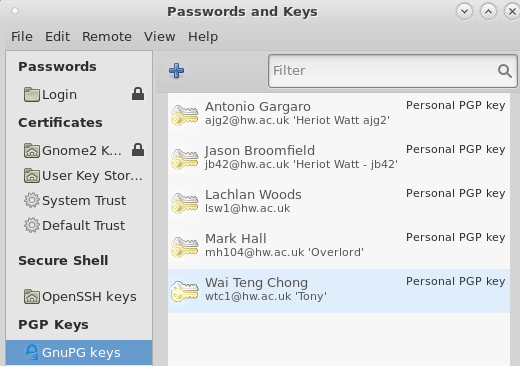
\includegraphics[width=0.45\textwidth]{imgs/key_signing/pass_keys_gui.PNG}} 
	\hfill
	\subfloat[Technical Overview]{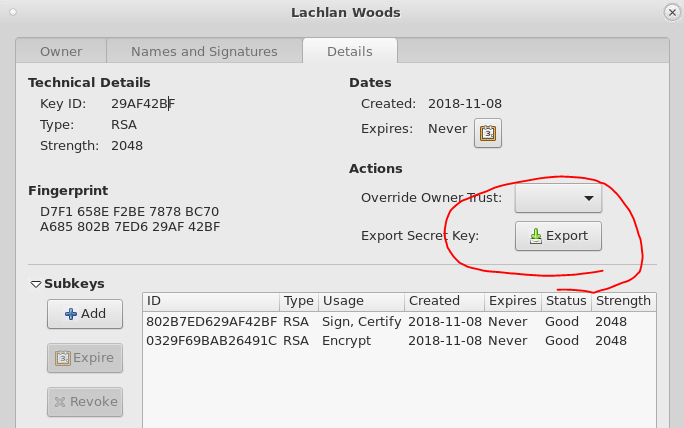
\includegraphics[width=0.5\textwidth]{imgs/key_signing/signed_private_key_export.PNG}} 
	\caption{Signing Lachlan's, Mark's and Tony's PGP key}
	\label{fig:key_part:keys_nd_pass}
    \noindent\makebox[\linewidth]{}
\end{figure}